\section{Critique and Potential Improvements}
In this section, we will discuss certain elements of the paper that we believe could be improved.

\subsection{Spherical Harmonics}
\label{sec:spherical_harmonics}
In the current implementation, they use spherical harmonics to handle view-dependent color from reflections.
They present this approach as "following standard practice" referencing the Plenoxels and Instant Neural Graphics papers \cite{yuPlenoxelsRadianceFields2021a}\cite{mullerInstantNeuralGraphics2022}.
As the paper uses a fundamentally different representation of the scene, I believe following the same approach for view-dependent color might not be the best choice.

The other methods both use some voxel-based representation of the scene,
where the sampling of each point is independent of the view direction,
making it necessary for each point to contain view-dependent color \cite{yuPlenoxelsRadianceFields2021a}\cite{mullerInstantNeuralGraphics2022}.
In the Gaussian splatting method, a discrete set of Gaussians is used to represent the scene, which could be leveraged to avoid the need for view dependence, by having overlapping Gaussians with view-dependent opacity.
This could be used to have Gaussians that are only visible from a narrow range of view directions, placed in front of the scene geometry to simulate reflections.

The paper shows that even without spherical harmonics, the scene converges to a good result \cite[Table 3]{kerbl3DGaussianSplatting2023}.
We propose to remove the spherical harmonic coefficients from the representation of each Gaussian, reducing the parameter number from 60 to 15 and adding a second phase to the rendering pipeline to handle reflections.
In this phase, we keep the converged scene constant and add a set of Gaussians with a view-dependent opacity to simulate reflections.

A potential problem with this approach is the popping effect discussed in Section \ref{sec:popping}, which makes it difficult to optimize Gaussians laying on the surface of the scene geometry.

\begin{figure}
    \centering
    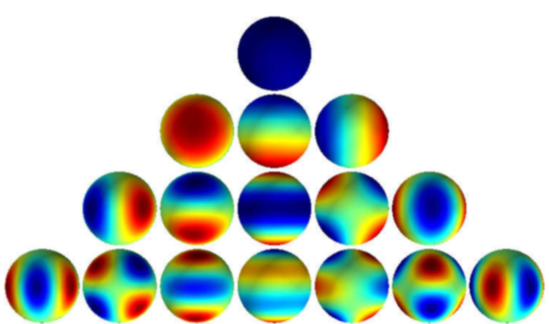
\includegraphics[width=\linewidth]{images/spherical_harmonics.png}
    \label{fig:spherical_harmonics}
    \caption{Visualization of the spherical harmonics used to represent the view-dependent color of each Gaussian \cite{pokorny2014a}.}
\end{figure}

\subsection{Use CUDA Streams to increase parallelism}
The code provided by the authors showcases a deep understanding of CUDA and GPU architecture,
notably in the way they ensure memory coalescing, avoid bank conflicts and leverage shared memory in the rasterization pipeline.
This makes it surprising that they do not use CUDA streams to increase parallelism.
When running the code on a workstation with an i9-13900KF CPU and an RTX 4090 GPU the GPU utilization was only around 30\% as the training process was severely bottlenecked by the single-threaded CPU code.
In the paper, they acknowledge that the majority (~80\%) of the training time is spent in Python code, and argue it is a necessary tradeoff to allow for easy adoption by other researchers \cite[Sec. 8]{kerbl3DGaussianSplatting2023}.
While the adaptability of the code is appreciated, it does not explain why they did not use CUDA Streams to increase parallelism, as Streams have deep support in PyTorch and can easily be disabled even if support is implemented \cite{pytorchcontributorsCUDASemanticsPyTorch2023}.

\subsection{Regularization}
The paper acknowledges that the optimized Gaussians tend to be very non-isotropic, i.e. very stretched out, as  Regularization is not performed \cite[Sec. 7.4]{kerbl3DGaussianSplatting2023}.
This is illustrated in Figure \ref{fig:very_isotropic}.
One way to solve this would be to add a cost based on the index of dispersion of the scale parameters $\bm{s}$ of each Gaussian, that is the ratio of the variance to the mean, which would have a value of 0 for spherical Gaussians.

\begin{figure}
    \centering
    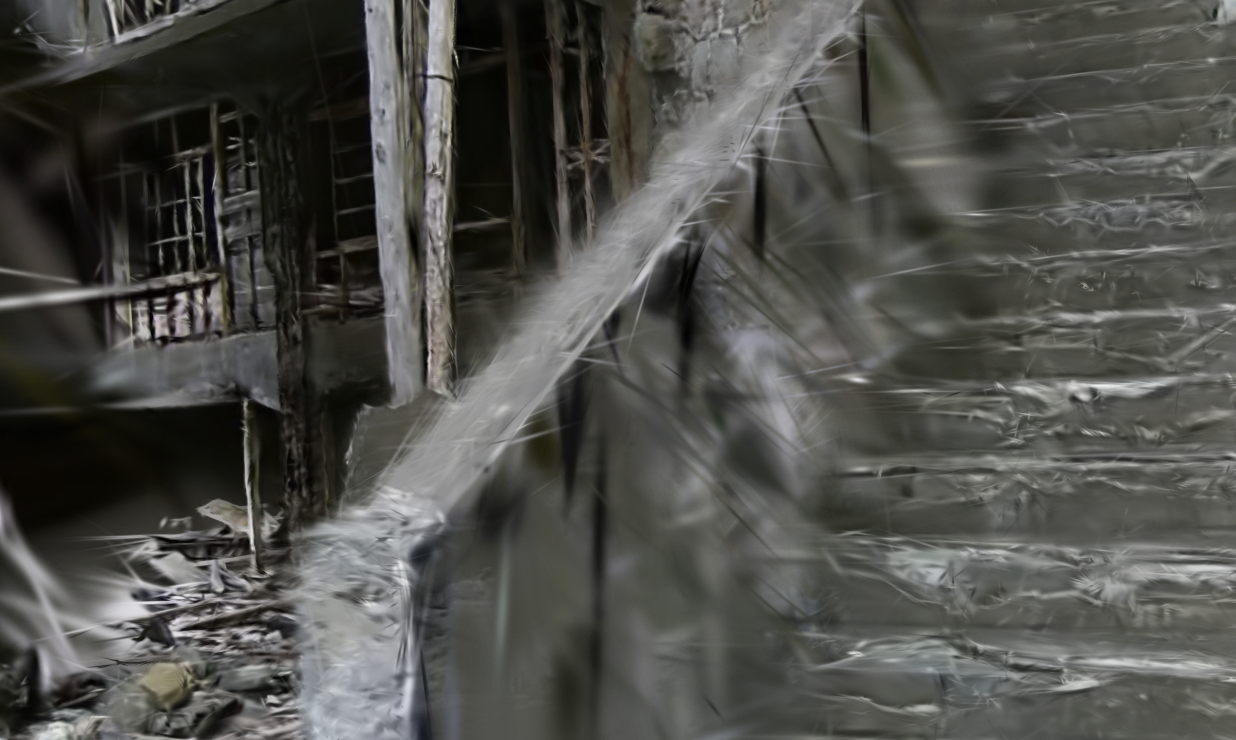
\includegraphics[width=\linewidth]{images/very_isotropic.png}
    \caption{Going outside the captured view angles illustrate how non-isotropic the Gaussians are \cite{@nekoHashimaIslandCreated2023}}
    \label{fig:very_isotropic}
\end{figure}

\subsection{Gaussian}
Why they chose to use a Gaussian to represent the scene is not explained in the paper.
As there is no connection to statistics or probability theory, it seems like an arbitrary choice.

